\documentclass{zkdl-tests-template}

\title{\huge\sffamily\bfseries Lecture \#6 Exercises}
\author{\Large\sffamily Distributed Lab}
\date{\sffamily August 22, 2024}
\titlepic{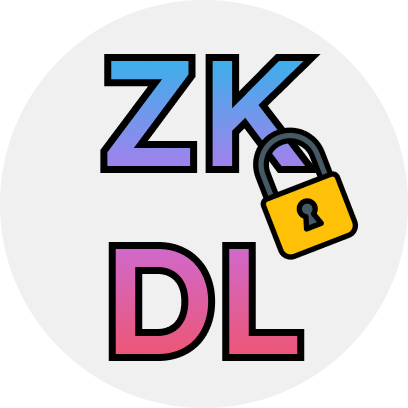
\includegraphics[width=0.15\textwidth]{../lectures/images/logo.png}}

\begin{document}

\pagestyle{fancy}

\maketitle

\textbf{Exercise 1.} When dealing with RSA protocol, one frequently encounters the following relation where $e$ is a prime number and $n \in \mathbb{N}$:
\begin{equation*}
    \mathcal{R} = \left\{ (w, x) \in \mathbb{Z}_n^{\times} \times \mathbb{Z}_n^{\times}: w^e = x \right\}
\end{equation*}

Which of the following is the language $\mathcal{L}_{\mathcal{R}}$ that corresponds to the relation $\mathcal{R}$?
\begin{enumerate}[(A)]
    \item Integers from $\mathbb{Z}_n^{\times}$ which have a modular root of $e$-th degree.
    \item Integers from $\mathbb{Z}_n^{\times}$ which are divisible by $e$.
    \item Integers $x$ from $\mathbb{Z}_n^{\times}$ with properly defined expression $x^e$.
    \item Integers from $\mathbb{Z}_n^{\times}$ which are prime.
    \item Integers from $\mathbb{Z}_n^{\times}$ for which $e$ is a primitive root.
\end{enumerate}

\textbf{Exercise 2.} Suppose that for some interactive protocol $(\mathcal{P}, \mathcal{V})$ during one round, the probability that the verifier $\mathcal{V}$ accepts a false statement is $1/8$. How many rounds of interaction are needed to guarantee $120$ bits of security? Assume here that $n$ bits of security means that the probability of accepting a false statement is at most $2^{-n}$.
\begin{enumerate}[(A)]
    \item $30$.
    \item $40$.
    \item $60$.
    \item $90$.
    \item $120$.
\end{enumerate}

\pagebreak
\textbf{Exercise 3.} Recall that for relation $\mathcal{R} = \{(w,x) \in \mathbb{Z}_N^{\times} \times \mathbb{Z}_N^{\times}: x = w^2\}$ we defined the following interactive protocol $(\mathcal{P}, \mathcal{V})$ to prove that $x \in \mathcal{L}_{\mathcal{R}}$:
\begin{itemize}
    \item $\mathcal{P}$ samples $r \xleftarrow{R} \mathbb{Z}_N^{\times}$ and sends $a = r^2$ to $\mathcal{V}$.
    \item $\mathcal{V}$ sends a random bit $b \in \{0,1\}$ to $\mathcal{P}$.
    \item $\mathcal{P}$ sends $z = r \cdot w^b$ to $\mathcal{V}$.
    \item $\mathcal{V}$ accepts if $z^2 = a \cdot x^b$, otherwise it rejects.
\end{itemize}

Suppose we use the protocol $(\mathcal{P}, \mathcal{V}^*)$ where the ``broken'' verifier $\mathcal{V}^*$ always outputs $b=1$. Which of the following statements is true?
\begin{enumerate}[(A)]
    \item Both the soundness and completeness of the protocol are preserved.
    \item The soundness of the protocol is preserved, but the completeness is broken.
    \item The completeness of the protocol is preserved, but the soundness is broken.
    \item Both the soundness and completeness of the protocol are broken.
\end{enumerate}

\textbf{Exercise 4.} What is the difference between the cryptographic proof and the proof of knowledge?
\begin{enumerate}[(A)]
    \item Cryptographic proof is a proof of knowledge that is secure against malicious verifiers.
    \item Cryptographic proof is a proof of knowledge that is secure against malicious provers.
    \item Cryptographic proof merely states the correctness of a statement, while the proof of knowledge also guarantees that the prover knows the witness.
    \item While cryptographic proof states that witness exists for the given statement, the proof of knowledge makes sure to make this witness unknown to the verifier.
    \item Proof of knowledge does not require verifier to know the statement, while cryptographic proof does.
\end{enumerate}

\textbf{Exercise 5.} What is the purpose of introducing the extractor?
\begin{enumerate}[(A)]
    \item To introduce the algorithm that simulates the malicious verifier trying to extract the witness from the prover.
    \item To define what it means that the prover knows the witness.
    \item To give the verifier the ability to extract the witness from the prover during the interactive protocol.
    \item To define the security of the interactive protocol that uses a more powerful verifier that can extract additional information from the prover.
    \item To give prover more power to extract randomness generated by the verifier.
\end{enumerate}

\pagebreak
\textbf{Exercise 6.} What it means that the interactive protocol $(\mathcal{P}, \mathcal{V})$ is a zero-knowledge?
\begin{enumerate}[(A)]
    \item The verifier $\mathcal{V}$ cannot know whether the given statement is true or false.
    \item The verifier $\mathcal{V}$ cannot know whether the prover $\mathcal{P}$ knows the witness.
    \item View of the prover $\mathcal{P}$ in the protocol is indistinguishable from the view of the verifier $\mathcal{V}$.
    \item Any view of any verifier $\mathcal{V}$ can be simulated using some polynomial-time algorithm, outputting computationally indistinguishable distribution from the given view.
    \item The prover $\mathcal{P}$ can convince the verifier $\mathcal{V}$ that the statement is true without knowing the witness.
 \end{enumerate}

\textbf{Hint:} View of the participant in the protocol consists of all data he has access to during the protocol execution. For example, verifier $\mathcal{V}$'s view consists of the messages he sends and receives, as well as the random coins he generates.

\textbf{Exercise 7.} Which of the following is \textbf{not} true about the Fiat-Shamir heuristic?
\begin{enumerate}[(A)]
    \item If the public-coin protocol is sound, the Fiat-Shamir transformation preserves the soundness.
    \item The Fiat-Shamir heuristic does not break the completeness of the public-coin protocol it is applied to.
    \item Practically, it allows to convert any interactive protocol into a non-interactive one.
    \item To make Fiat-Shamir transformation pratical, the function modelling the random oracle should be hard to invert.
    \item It is reasonable to use SHA256 to model the random oracle in the Fiat-Shamir transformation.
\end{enumerate}

\end{document}
